\subsection{Equalizing}
The audible frequencies can be separated into octaves. An octave is an interval between to frequencies, where the the highest frequency is double the frequency of the lowest frequency. Companies, such as Dolby Lake \citep{lab_gruppen_eq}, now owned by Music group and Powersoft \citep{powersoft_eq}, separates their equalizing bands in thirds of an octave. 
The \gls{eq} is made with a bank of bandpass filters, using either octave or third octave separation from \SI{20}{\hertz} to \SI{20}{\kilo\hertz}, but the octave order can be changed in advanced systems. Both analog and digital \gls{eq}s normally use octave or third octave separation. These bandpass filters are able to either amplify or attenuate the gain of the specified frequency. The \autoref{fig:analog_equalizer} shows an analog \gls{eq} with traditional third octave separation \citep{nordic}

\begin{figure} [htbp]
 \centering
  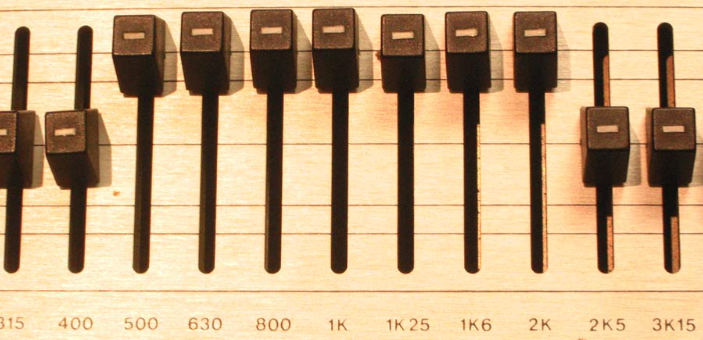
\includegraphics[width=0.6\textwidth]{analog_equalizer}
  \caption{The photo shows an example of an analog equalizer \citep{nordic}.}
  \label{fig:analog_equalizer}
\end{figure}

\todo[inline]{Mohamed : Maybe add why they will affect each other}
One amplified bandpass filter will interfere with the neighbouring filters, thus the frequency response will be different than what can be expected with ideal filters. The following \autoref{fig:analog_equalizer_respond} shows the frequency response of the above analog \gls{eq} \autoref{fig:analog_equalizer}.

\begin{figure} [htbp]
 \centering
  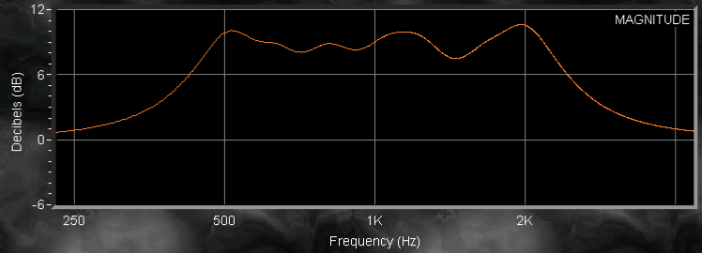
\includegraphics[width=0.8\textwidth]{analog_equalizer_respond}
  \caption{The photo shows the response of the equalizer at \autoref{fig:analog_equalizer} \citep{nordic}.}
  \label{fig:analog_equalizer_respond}
\end{figure}

A simple block diagram of a \gls{eq}  is shown in the following \autoref{fig:equalizer_block}.

\begin{figure}[htb] 
	\begin{center} 
\begin{picture}(0,0)%
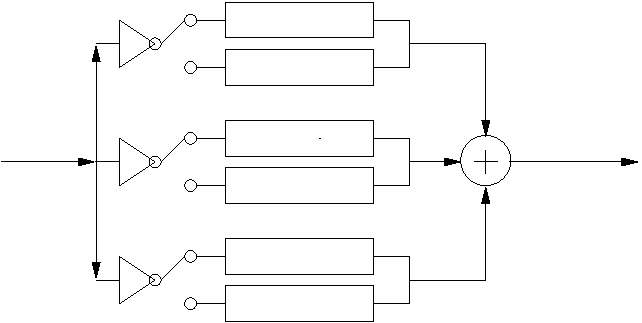
\includegraphics{eq.pdf}%
\end{picture}%
\setlength{\unitlength}{4144sp}%
%
\begingroup\makeatletter\ifx\SetFigFont\undefined%
\gdef\SetFigFont#1#2#3#4#5{%
	\reset@font\fontsize{#1}{#2pt}%
	\fontfamily{#3}\fontseries{#4}\fontshape{#5}%
	\selectfont}%
\fi\endgroup%
\begin{picture}(4344,2454)(3319,-658)
\put(6796,749){\makebox(0,0)[lb]{\smash{{\SetFigFont{12}{14.4}{\rmdefault}{\mddefault}{\updefault}{\color[rgb]{0,0,0}Output}%
}}}}
\put(5086,1244){\makebox(0,0)[lb]{\smash{{\SetFigFont{5}{6.0}{\rmdefault}{\mddefault}{\updefault}{\color[rgb]{0,0,0}1st Inverse}%
}}}}
\put(5086,1604){\makebox(0,0)[lb]{\smash{{\SetFigFont{7}{8.4}{\rmdefault}{\mddefault}{\updefault}{\color[rgb]{0,0,0}1st Band}%
}}}}
\put(5086,704){\makebox(0,0)[lb]{\smash{{\SetFigFont{7}{8.4}{\rmdefault}{\mddefault}{\updefault}{\color[rgb]{0,0,0}2nd Band}%
}}}}
\put(5131,-196){\makebox(0,0)[lb]{\smash{{\SetFigFont{7}{8.4}{\rmdefault}{\mddefault}{\updefault}{\color[rgb]{0,0,0}3rd Band}%
}}}}
\put(5131,-556){\makebox(0,0)[lb]{\smash{{\SetFigFont{5}{6.0}{\rmdefault}{\mddefault}{\updefault}{\color[rgb]{0,0,0}3rd Inverse}%
}}}}
\put(5086,344){\makebox(0,0)[lb]{\smash{{\SetFigFont{5}{6.0}{\rmdefault}{\mddefault}{\updefault}{\color[rgb]{0,0,0}2nd Inverse}%
}}}}
\put(3421,749){\makebox(0,0)[lb]{\smash{{\SetFigFont{12}{14.4}{\rmdefault}{\mddefault}{\updefault}{\color[rgb]{0,0,0}Input}%
}}}}
\end{picture}%

			\caption{This figure shows a simple block diagram over a \gls{eq}.} \label{fig:equalizer_block} 
			\end{center}
			\end{figure}


The block diagram \autoref{fig:equalizer_block} shows an simple equalizer, where each bandpass filter is divided into separate blocks. Each block is separated by octaves, where the next higher bandpass filter frequency is raised by a factor 2. 

